% Asset ID: AS2StatisticalDistributionsTikZ-002
% Source: Chapter 6 Statistical Distributions transcript, binomial distribution definition
% Related lesson section: Core Theory 8.4 and Exam Technique Notes
% Purpose: Binomial model conditions checklist.

\documentclass[tikz,border=8pt]{standalone}
\usepackage{amsmath}
\usetikzlibrary{positioning, arrows.meta}

\begin{document}
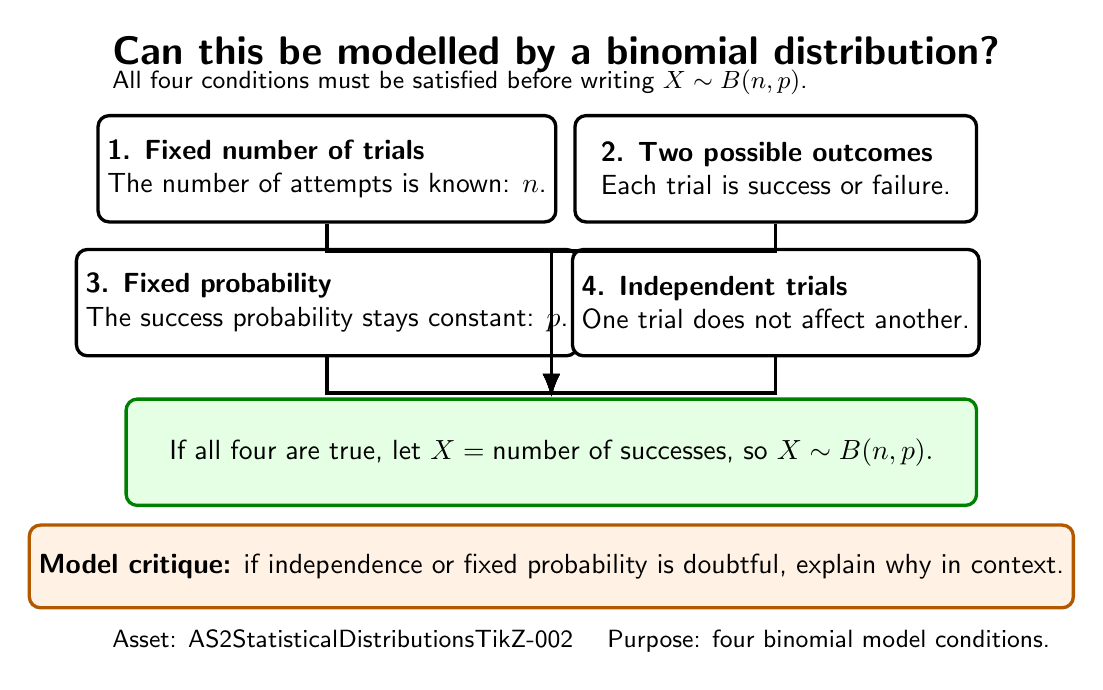
\begin{tikzpicture}[box/.style={draw=black,very thick,rounded corners,fill=white,minimum width=5.1cm,minimum height=1.35cm,align=left,font=\sffamily},good/.style={draw=green!50!black,very thick,rounded corners,fill=green!10,minimum width=10.8cm,minimum height=1.35cm,align=center,font=\sffamily},warn/.style={draw=orange!70!black,very thick,rounded corners,fill=orange!10,minimum width=10.8cm,minimum height=1.05cm,align=center,font=\sffamily},arrow/.style={very thick, -{Latex[length=3mm]}},title/.style={font=\sffamily\bfseries\Large},subtitle/.style={font=\sffamily\small}]
\node[anchor=west, title] at (-5.7,3.4) {Can this be modelled by a binomial distribution?};
\node[anchor=west, subtitle] at (-5.7,3.05) {All four conditions must be satisfied before writing $X\sim B(n,p)$.};
\node[box] (fixed) at (-2.85,1.95) {\textbf{1. Fixed number of trials}\\The number of attempts is known: $n$.};
\node[box] (two) at (2.85,1.95) {\textbf{2. Two possible outcomes}\\Each trial is success or failure.};
\node[box] (prob) at (-2.85,0.25) {\textbf{3. Fixed probability}\\The success probability stays constant: $p$.};
\node[box] (ind) at (2.85,0.25) {\textbf{4. Independent trials}\\One trial does not affect another.};
\node[good] (model) at (0,-1.65) {$\displaystyle \text{If all four are true, let } X=\text{number of successes, so } X\sim B(n,p).$};
\draw[arrow] (fixed.south) -- ++(0,-0.35) -| (model.north);
\draw[arrow] (two.south) -- ++(0,-0.35) -| (model.north);
\draw[arrow] (prob.south) -- ++(0,-0.45) -| (model.north);
\draw[arrow] (ind.south) -- ++(0,-0.45) -| (model.north);
\node[warn] at (0,-3.1) {\textbf{Model critique:} if independence or fixed probability is doubtful, explain why in context.};
\node[anchor=west, subtitle] at (-5.7,-4.05) {Asset: AS2StatisticalDistributionsTikZ-002 \quad Purpose: four binomial model conditions.};
\end{tikzpicture}
\end{document}
